\documentclass{pracamgr}

\usepackage{polski}

\usepackage[utf8]{inputenc}
\usepackage[T1]{fontenc}
\usepackage{algorithm}
\usepackage[noend]{algpseudocode}
\usepackage{amsmath}
\usepackage{graphicx}
\usepackage{tikz}
\usepackage{verbatim}
\usepackage{enumitem}
\usepackage[title,titletoc]{appendix}
\usepackage[labelfont=bf]{caption}
\usepackage{float}

\floatstyle{boxed}
\newfloat{algorytm}{h}{}
\floatname{algorytm}{Algorytm}

\floatstyle{plain}
\newfloat{rysunek}{h}{}
\floatname{rysunek}{Rysunek}

\floatstyle{plain}
\newfloat{tabela}{h}{}
\floatname{tabela}{Tabela}


% version header
\usepackage{fancyhdr}
\pagestyle{fancy}
\fancyhead{}
\fancyhead[C]{wersja 4}

\fancypagestyle{plain}{%
}
\fancypagestyle{empty}{%
}
%%% version head


\usetikzlibrary{arrows}

\graphicspath{{img/}}

\author{Bartosz Marcinkowski}

\nralbumu{319476}

\title{Sztuczna inteligencja dla gier planszowych na przykładzie Quoridor}
\tytulang{Artificial intelligence for board games in the example of Quoridor}

\kierunek{Informatyka}

\opiekun{prof. Jana Madeya}

\date{Maj 2017}

\dziedzina{11.3 Informatyka}

\klasyfikacja{
I. Computing Methodologies \\
  I.2. Artificial intelligence \\
  I.2.1. Applications and Expert Systems}

\keywords{
	sztuczna inteligencja, gry planszowe, minimax, Monte-Carlo Tree Search, Quoridor
}

% Tu jest dobre miejsce na Twoje własne makra i~środowiska:
\newtheorem{defi}{Definicja}[section]

% koniec definicji

\begin{document}
\maketitle

\begin{abstract}
W pracy zajmiemy się algorytmami sztucznej inteligencji dla gier planszowych.
Opiszemy podstawowe metody, ze szczególnym uwzględnieniem liczby graczy jako czynnika wpływającego na użyteczność algorytmu.
Dalej, przejdziemy do możliwych ulepszeń, zarówno ogólnych i specyficznych dla gry Quoridor, na której się skupimy.
Przedstawimy też implementację opracowanych metod na potrzeby wytwarzanego prototypu aplikacji, dzięki której użytkownik będzie mógł eksperymentować z różnymi algorytmami.
\end{abstract}

\tableofcontents
%\listoffigures
%\listoftables


\chapter{Wprowadzenie}

\section{Tematyka pracy}

W pracy zajmiemy się algorytmami sztucznej inteligencji dla gier planszowych.
Tego określenia używamy jako intuicyjnej nazwy pewnej klasy gier, która niekoniecznie pokrywa się dokładnie ze zbiorem gier korzystających z planszy.
Obejmuje ona w szczególności warcaby, szachy, go i stanowi obiekt zainteresowania informatyki przynajmniej od roku 1949 (por. \cite{anderson}), kiedy Claude Shannon napisał pracę \textit{Programming a Computer for Playing Chess}.
Przez wiele lat to właśnie gra w szachy stanowiła jeden z wyznaczników stanu zaawansowania sztucznej inteligencji, obok m. in. testu Turinga.
Na drodze do spektakularnego sukcesu z 1997 roku, kiedy superkomputer Deep Blue pokonał wielokrotnego mistrza świata Garri Kasparowa, prace nad programami grającymi w szachy przynosiły wyniki bardziej ogólne, dające się zastosować do innych gier.
Tak powstawały niektóre metody uznawane dziś za standardowe.

W tej pracy również skupimy zainteresowanie na jednej grze --- Quoridor --- która mimo prostych zasad dorównuje złoźonością szachom (por. \cite{mertens}).
Mamy nadzieję, że i nam uda się uzyskać efekty interesujące dla osób zajmujących się innymi grami.
Poszukiwania zaczniemy od przeglądu powszechnie stosowanych, podstawowych metod oraz wybranych ulepszeń, które będą wydawać się przydatne dla Quoridor.
Opiszemy ich wykorzystanie lub dostosowanie i próby ulepszenia, a także porównamy między sobą.
Później postaramy się z naszych wysiłków wyłuskać efekty ogólne, dające się zastosować poza Quodior.

Równolegle z pracą będziemy wytwarzać oprogramowanie otwartoźródłowe --- prototyp komputerowej wersji gry, która będzie umożliwiać użytkownikowi mierzenie się z różnymi algorytmami sztucznej inteligencji albo obserwację rozgrywek między nimi.
Użytkownikowi-programiście, naturalnemu odbiorcy prototypu z publicznym dostępem do kodu, ma umożliwiać modyfikowanie i dodawanie algorytmów oraz porównywanie poprzez przeprowadzanie automatycznych turniejów.
Aplikacja, jako bezpośrednia motywacja do poszukiwań teoretycznych, pomoże wyznaczyć dla nich wymagania i ograniczenia.

Zwrócimy też uwagę na często pomijany, ale istotny dla gry komputerowej, aspekt algorytmu sztucznej inteligencji dla gier planszowych --- wpływ na jakość interakcji z użytkownikiem.
A więc w miarę możliwości będziemy starać się, żeby gracz komputerowy spośród wielu możliwych sposobów uzyskania takiego samego efektu wybrał taki sposób, który uczyni rozgrywkę najbardziej przyjemną dla przeciwnika.

\section{Quoridor --- oryginalne zasady gry}

Gra rozgrywa się na planszy za pomocą 4 pionków i 20 ogrodzeń, nazywanych też \emph{ścianami}. Na planszy znajduje się siatka szczelin wyznaczająca 81 kwadratowych pól, tworzących układ 9~x~9. Każdy pionek ma unikatowy kolor, mieści się na jednym polu planszy i nie może go dzielić z innym. Ogrodzenia są identyczne i dają się umieszczać w szczelinach między polami planszy. Ogrodzenie jest dwukrotnie dłuższe od boku pola, więc (poprawnie umieszczone) sąsiaduje z dwoma polami z każdej strony, zajmuje całą szerokość szczeliny i jedno skrzyżowanie szczelin.

W grze może wziąć udział dwóch lub czterech graczy. W obu przypadkach otrzymują po jednym pionku, dzielą się po równo ogrodzeniami i przypisują się do różnych boków planszy; jeżeli jest ich dwóch, muszą to być boki przeciwległe.

Na początku gry na planszy nie ma ogrodzeń (stanowią one zasoby graczy), a pionek każdego gracza umieszcza się na polu przy środku boku, do którego jest przypisany.
Następnie gracze wykonują kolejno swoje ruchy. Celem gry jest dotarcie swoim pionkiem do boku planszy przeciwległego wobec boku, do którego jest się przypisanym. Gra kończy się w momencie, w którym jednemu z graczy się to uda.

Każdy ruch polega na ustawieniu jednego ze swoich nieużytych ogrodzeń na planszy albo przesunięciu pionka. Ogrodzenie nie może kolidować z żadnym innym i nie może odciąć żadnemu graczowi wszystkich dróg do celu. Ruch pionkiem polega na przesunięciu go na puste, sąsiadnie pole (sąsiedztwo wyznacza wspólny bok).

Jeżeli na pewnym sąsiednim, nieodgrodzonym polu znajduje się już pionek przeciwnika, można wykonać skok na pole za tym pionkiem, o ile jest ono puste i nieodgrodzone. Jeżeli taki skok nie jest możliwy, można wykonać skok na jedno z dwóch pozostałych pól sąsiadujących z przeciwnikiem, znów o ile jest puste i nieodgrodzone.

\section{Cele i założenia}

Opracowywanie sztucznej inteligencji do gier planszowych może mieć różne założenia i cele.
Nie interesują nas tu metody wymagające mocy obliczeniowej superkomputera.
Celem tej pracy jest opracowanie algorytmów sztucznej inteligencji dla gry Quoridor i utworzenie prototypu oprogramowania otwartoźródłowego, łatwego w dystrybucji i nadającego się do użycia na komputerze osobistym lub urządzeniu przenośnym, które będzie umożliwało grę w obu wariantach gry (dla 2 i 4 graczy), przy czy każdy gracz może być człowiekiem albo graczem komputerowym sterowanym przez jeden z dostępnych algorytmów sztucznej inteligencji.

\section{Istniejące rozwiązania}

Dostępnych jest już kilka programów grających w Quoridor. Są to aplikacje działające w przeglądarce internetowej lub na urządzeniu przenośnym. Żadna z nich nie osiąga celów, jakie postawiliśmy tworzonemu przez nas oprogramowaniu.
Tylko w jednym przypadku\footnote{http://danielborowski.com/quoridor-ai/v2/display.html} udostępniony jest kod źródłowy.
Inna aplikacja\footnote{https://play.google.com/store/apps/details?id=com.codestare.corridor}, wciąż w trakcie rozwoju, jest jedyną implementująca oba warianty gry.

\section{Struktura pracy}

W drugim rozdziale określimy szerszą klasę gier, w której znajduje się Quoridor.
Wprowadzimy pojęcia używane do ich opisu i algorytmy sztucznej inteligencji, które są wobec nich standardowo stosowane.

W trzecim rozdziale określimy te aspekty aplikacji, którę są istotne dla graczy komputerowych (dalej ,,botów'').
Tak więc doprecyzujemy zasady gry, wybierzemy technologie, zdefiniujemy interfejs bota, ograniczenia wykorzystania zasobów i oczekiwany czas działania.

W czwartym rozdziale opiszemy proces rozwijania kolejnych algorytmów.
Uzasadnimy wybór tych, które zaimplementujemy, wymienimy napotykane problemy oraz przedstawimy nasze rozwiązania.

W piątym rozdziale podsumujemy efekty naszej pracy.
Wskażemy kierunki dalszego ulepszania stworzonych botów i spróbujemy wyciągnąć wnioski przydatne przy implentacji komputerowych wersji innych gier.

\chapter{Standardowe metody dla stosownej klasy gier}

\section{Klasyfikacja Quoridor}

Żeby poznać stan wiedzy na temat sztucznej inteligencji w grach takich jak Quoridor, musimy najpierw określić tę klasę gier.
Cechy gry mające decydujący wpływ na algorytmy sterujące botami to:

 - podział na tury lub ciągłe wykonywanie ruchów,

 - pełna lub niepełna informacja o stanie gry,

 - istnienie elementów losowości,

 - podział zysku,

 - liczba graczy.

Na wyjaśnienie zasługuje tu ,,podział zysku''.
Ta cecha gry określa sposób, w jaki gracze są nagradzani, w szczególności decyduje o tym, czy jest opłacalna kooperacja. I tak na przykład szachy, są grą o sumie stałej, tzn. korzyść przeciwnika jest jednoznaczna ze stratą. Inaczej bywa w grach ekonomicznych, gdzie współpraca między graczami może zwiększyć wypłatę nagrody dla obu graczy.

Quoridor jest grą z podziałem na tury, z pełną informacją o stanie gry, bez losowości i jest grą o sumie stałej.
A więc w wariancie dla dwóch graczy znajduje się w tej samej klasie gier co szachy, warcaby, go i wiele innych klasycznych gier, którymi informatyka zajmuje się od dziesięcioleci.
Wiele z metod dla tej klasy gier zasłużyło już na miano standardowych.

Wariant dla czterech graczy wciąż pozostaje pod wieloma względami podobny do gier klasycznych.
Nie ma osobnego zestawu standardowych metod dla tego przypadku, który moglibyśmy tu przedstawić.
Stosuje się, o ile to możliwe, specjalne warianty algorytmów używanych dla dwóch graczy.

Od tej pory będziemy mówić wyłącznie o grach o sumie zerowej, z pełną informacją o stanie gry, w których gracze wykonują ruchy na zmianę.
Po wprowadzeniu podstawowych pojęć, zaprezentujemy metody standardowe (na podstawie~\cite{pawlewicz}), napierw specyficzne dla gier dwuosobowych (Minimax i Alfa-Beta), później niezależne od liczby graczy (Monte Carlo).
Na końcu przestawimy metody dostosowania algorytmów typowych dla gier dwuosobowych do gier z większą liczbą graczy.

\section{Podstawowe pojęcia}

Podstawową abstrakcją używaną do opisu gry jest graf skierowany, w którym wierzchołki reprezentują stany gry, a krawędzie odpowiadają legalnym ruchom.
Rozgrywka jest ścieżką, być może zawierającą cykle, od stanu początkowego do jednego ze stanów końcowych.

Na potrzeby algorytmów sztucznej inteligencji często wygodniej jest użyć drzewa gry, w którym wielu wierzchołkom może odpowiadać ten sam stan gry.
Stan, dla którego ma być wybrany kolejny ruch, jest reprezentowany przez korzeń, stany końcowe przez liście, a możliwy dalszy przbieg rozgrywki przez ścieżkę od korzenia do liścia.

W dalszej części pracy będziemy zamiennie używać pojęć stan i wierzchołek, ruch i krawędź itd. o ile nie będzie powodować to nieporozumień.

Kolejnym pojęciem pojawiającym się w tych algorytmach jest funkcja oceniająca.
Jest to funkcja przypisująca stanowi gry liczbę całkowitą, która ma oceniać jak bardzo pożądany jest ten stan dla danego gracza.
Powinna przyjmować skrajne wartości dla stanów końcowych (największą dla wygrywających, a najmniejszą dla przegrywających).

\section{Minimax i Alfa-Beta}

Algorytmy Minimax i Alfa-Beta zostały zaprojektowany z myślą o grach dwuosobowych.
W grze dwuosobowej o sumie zerowej przyjmujemy, że dla każdego stanu funkcja oceniająca jednego gracza przyjmie wartość przeciwną do funkcji oceniającej drugiego gracza.
A więc można wybrać jedną z tych funkcji oceniających jako jedyną interesującą.
Gracz, którego funkcja została wyróżniona nazywany jest wtedy \(max\), a jego przeciwnik \(min\).
Zgodnie z intuicją, gracz \(max\) wybiera stany maksymalizujące wartość wyróżnionej funkcji, a gracz \(min\) minimalizujące.

\subsection{Minimax}

Algorytm Minimax rozpatruje w drzewie gry tylko poddrzewo bieżącego stanu gry do ustalonej głębokości. W tak uzyskanym drzewie, liściom jest przypisana wartość funkcji oceniającej.
Pozostałe wierzchołki będą miały przypisywane wartości na podstawie wartości synów (patrz Algorytm \ref{minimax}).

\begin{algorytm}
\caption{Minimax\label{minimax}}
\begin{algorithmic}[1]
\Function{minimax}{$v$}
\If {$\texttt{\(v\) jest liściem}$}
	\State \Return $funkcjaOceniajaca(v)$
\EndIf
\If {$\texttt{ruch wykonuje gracz \(max\)}$}
    \State \Return $max$($minimax(w) | \texttt{\(w\) jest synem \(v\)})$
\Else
    \State \Return $min$($minimax(w) | \texttt{\(w\) jest synem \(v\)})$
\EndIf
\EndFunction
\end{algorithmic}
\end{algorytm}

Znając wartości \(minimax\) dla synów korzenia, możemy wybrać najkorzystniejszy ruch dla obecnego gracza.

\subsection{Alfa-Beta}

Algorytm Alfa-Beta jest ulepszeniem algorytmu minimax.
Opiera się na następującej obserwacji: wartości \(minimax\) niektórych wierzchołków mogą być ustalone bez obliczania ich dla wszystkich potomków aż do liści, a więc niektóre poddrzewa mogą zostać ,,odcięte'' (przykład na Rysunku \ref{alfa-beta-cut}).
Oszczędzając w ten sposób czas można zwiększyć głębokość przeszukiwanego drzewa, a więc podjąć lepszą decyzję.

\begin{rysunek}
\caption{Odcięcie w algorytmie Alfa-Beta \label{alfa-beta-cut}}
\centering
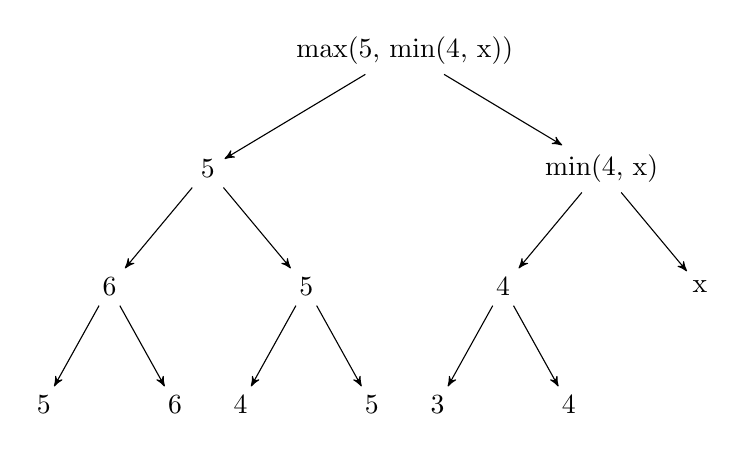
\begin{tikzpicture}[->,>=stealth',level/.style={sibling distance = 5cm/#1,
  level distance = 1.5cm}]
\node {max(5, min(4, x))}
    child{ node {5}
    	child{ node {6}
            child{ node {5}}
            child{ node {6}}
        }
		child{ node {5}
            child{ node {4}}
            child{ node {5}}
        }
    }
    child{ node {min(4, x)}
        child{ node {4}
            child{ node {3}}
            child{ node {4}}
        }
        child{ node {x}}
    }
;
\end{tikzpicture}

\end{rysunek}

Algorytm Alfa-Beta wprowadza pomocniczą funkcję \(alfabeta\):

\[
  \begin{cases}
    alfabeta(v, alfa, beta) \leq alfa    & \quad \text{if } minmax(v) \leq alfa\\
    alfabeta(v, alfa, beta) = minimax(v) & \quad \text{if } alfa < minmax(v) < beta \\
    alfabeta(v, alfa, beta) \geq beta    & \quad \text{if } minmax(v) \geq beta \\
  \end{cases}
\]

Przedział \((alfa, beta)\) jest nazywany \emph{oknem przeszukiwania} --- wartość wewnątrz niego to dokładnie obliczona wartosć \(minimax\).
Dla korzenia za okno przeszukiwania przyjmuje się przedział \((-\infty, \infty)\), a więc oblicza się dokładną wartość \(minimax\).
Znaczenie okna przeszukiwania można wyrazić następującą intuicją: jeżeli wartość obliczana dla danego wierzchołka jest większa niż \(beta\), to końcowy wynik obliczeń nie zmieni się, jeżeli za wartość bieżącego wierzchołka przyjmiemy \(beta\) lub dowolną większą liczbę; gracz \(min\) nie dopuści do rozpatrywanego stanu, ponieważ ma lepszą alternatywę.
Analogicznie, gdy wartość jest mniejsza niż \(alfa\), dla gracza \(max\) (patrz Algorytm \ref{alfabeta}).

\begin{algorytm}
\caption{Alfa-Beta\label{alfabeta}}
\begin{algorithmic}[1]
\Function{alfabeta}{$v, alfa, beta$}
\If {$\texttt{\(v\) jest liściem}$}
	\State \Return $funkcjaOceniajaca(v)$
\EndIf
    \If {\texttt{ruch wykonuje gracz \(max\)}}
    \ForAll {\texttt{\(w\) jest synem \(v\)}}
        \State $alfa \gets max(alfa, alfabeta(w, alfa, beta))$
        \If {$ alfa \geq beta$}
            \State \textbf{break}
        \EndIf
    \EndFor
	\State \Return $alfa$
\Else
    \ForAll {\texttt{\(w\) jest synem \(v\)}}
        \State $beta \gets min(beta, alfabeta(w, alfa, beta))$
        \If {$ alfa \geq beta$}
            \State \textbf{break}
        \EndIf
    \EndFor
	\State \Return $beta$
\EndIf
\EndFunction
\end{algorithmic}
\end{algorytm}

\subsection{Tablica transpozycji}

Ponieważ algorytmy Minimax i Alfa-Beta traktują graf gry jako drzewo, ten sam wierzchołek może być odwiedzony kilkukronie, o ile prowadzą do niego różne ścieżki.
Ta obserwacja jest podstawą techniki tablicy transpozycji, która pozwala na wykorzystanie wyników wcześniejszych obliczeń w trakcie działania algorytmu i przyspieszenie, dzięki któremu można zwiększyć głębokość przeszukiwania.

Zastosowanie tablicy transpozycji wymaga użycia funkcji haszującej \(h\), która umożliwi przypisanie każdemu stanowi gry liczbę całkowitą, ograniczoną z góry przez ustaloną wartość.
Należy też ustalić wielkość tablicy \(R\), która będzie musiała zmieścić się w pamięci dostępnej botowi.
Wtedy, po obliczeniu wartości wierzchołka \(w\), pod indeksem \(h(w)\ \textrm{mod}\ R\) tablicy haszującej umieszcza się wpis zawierający \(h(w)\), odległość wierzhołka \(w\) od korzenia w przeszukiwanym drzewie (wysokość) oraz specyficzne dla algorytmu wartości przydatne przy ponownym odwiedzeniu wierzchołka \(w\).
Zapisana wartość \(h(w)\), podczas odwiedzania wierzchołka \(v\) takiego, że \(h(w) \equiv h(v) (\textrm{mod}\ R)\), pozwala rozpoznać kolizję.
Zapisana wysokość wierzchołka \(w\) określa jakość wpisu.
Wysokość równa głębokości przeszukiwania oznacza, że wierzchołek był odwiedzony jako liść i zapisana wartość jest wprost wartością funkcji oceniającej dla tego wierzchołka.
Taką wartość uznajemy za gorszą od obliczonej dla wysokości o jeden mniejszej, kiedy rozpatrzone zostały wszystkie możliwe kolejne ruchy.
A zatem odnaleziony w tablicy transpozycji wpis może zostać użyty tylko wtedy, gdy zgadzają się wartości funkcji haszującej oraz wysokość zapisana we wpisie jest nie większa niż bieżąca.

W przypadku algorymu Minimimax dodatkowym polem wpisu jest to po prostu obliczona wartość wierzchołka, która może zostać użyta po spełnieniu wcześniej wymienionych warunków.

W przypadku algorytmu Alfa-Beta, wpis zawiera ograniczenie dolne i górne na wartość \(minimax\) wierzchołka (równe sobie, jeżeli znana jest dokładna wartość).
Taki wpis nie zawsze pozwala natychmiast podać wynik, ale może zawęzić okno przeszukiwania i skrócić czas działania algorytmu.

\subsection{Inne ulepszenia}

Istnieją dalsze ulepszenia algorytmu Alfa-Beta (NegaScout, MTD-f), które opierają się na zawężaniu okna przeszukiwania.
Ten zabieg skraca czas działania, ale może nie dać przydatnego wyniku.
Na przykład, zamiast obliczać wartość \(alfabeta(w, alfa, beta)\) oblicza się \(alfabeta(w, alfa, beta')\), gdzie \(alfa < beta' < beta\).
Otrzymana wartość jest poprawnym wynikiem \(alfabeta(w, alfa, beta)\), o ile jest mniejsza od \(beta'\).
Choć obliczanie nieużytecznych wyników spowalnia algorytm, powinno zdarzać się rzadko.
Ostatecznie, skuteczność tych technik sprawdza się eksperymentalnie.

\section{Metody Monte Carlo}

Metoda Monte Carlo nie opiera się w żaden sposób na Minimax i w ogóle nie wymaga użycia funkcji oceniającej wartość wierzchołka.
Do jej zastosowania wystarczy znajomość zasad gry, to znaczy możliwych ruchów dla każdego stanu oraz stanów końcowych wraz z wynikiem rozgrywki.
Ruchy są oceniane na podstawie wyników losowych symulacji; w najprostszym algorytmie, od synów danego wierzchołka moglibyśmy rozpocząć równą liczbę losowych rozgrywek i wybrać tego, który najczęściej doprowadził do zwycięstwa.

\subsection{Monte Carlo Tree Search}

W praktyce prosta metoda Monte Carlo nie sprawdza się i należy w trakcie przeprowadzania symulacji niektóre wierzchołki początkowe porzucać jako mało obiecujące, a inne rozwijać, tzn. w ich miejsce wstawić wszystkich synów jako samodzielne wierzchołki początkowe symulacji.
Tak działa Monte Carlo Tree Search.

Algorytm ten utrzymuje drzewo, zakorzenione w wierzchołku dla którego wybiera ruch i początkowo posiadające ponad to wyłącznie liść dla każdego możliwego kolejnego stanu gry.
Każdy wierzchołek tego drzewa utrzymuje statystyki symulacji: liczbę symulacji i liczbę symulacji zakończonych zwycięstwem, które rozpoczęły się w poddrzewie danego wierzchołka.
Tak długo jak pozwalają na to limity czasu i pamięci, algorytm przechodzi od korzenia do pewnego liścia wybierając zawsze najbardziej obiecującego syna w zależności od wcześniej zebranych statystyk. Na podstawie statystyk liścia podejmuje decyzję o rozwinięciu go (dodaniu możliwych kolejnych stanów gry do drzewa ze statystykami) i jeśli to zrobi, wybiera jednego z dodanych synów, aby ostatecznie zawsze wybrać liść.
Dalej rozpoczyna od liścia losową rozgrywkę aż do poznania zwycięzcy, po czym aktualizuje statystyki wierzchołków na ścieżce od korzenia do liścia, z którego rozpoczęła się symulacja.
Najlepszy ruch z korzenia wyznacza jego syn, w którego statystykach stosunek zwycięstw do przeprowadzonych symulacji jest najkorzystniejszy.

W opisie algorytmu widać pewne luki: sposób wybierania najbardziej obiecującego syna i kryteria decyzji o rozwinięciu liścia.

Przy wybieraniu nabardziej obiecującego syna używa się metody granicy ufności.
Ma ona zapobiec sytuacji, w której po niewielkiej liczbie symulacji (nawet tylko jednej) liść jest porzucany, co ma miejsce gdy porównuje się wyłącznie stosunek liczby zwycięstw do liczby symulacji.
W tym celu to tego ilorazu jest dodawany \emph{współczynnik ufności}, tym wyższy im mniejszą częścią symulacji rodzica są symulacje danego syna. Jako współczynnik ufności przymuje się \(\sqrt{\frac{\sqrt{n_p}}{n_s}}\) lub \(\sqrt{\frac{\log{n_p}}{n_s}}\), gdzie \(n_s\) to liczba symulacji w poddrzewie syna, a \(n_p\) to liczba symulacji w poddrzewie rodzica.

Decyzję o rozwinięciu liścia podejmuje się na podstawie liczby symulacji, jakie zostały z niego rozpoczęte. Jeżeli przekroczy ustalony próg, zwykle zbliżony do liczby ruchów możliwych w jednym stanie gry, liść zostaje rozwinięty.

Oba parametry, tzn. wariant granicy ufności i próg rozwinięcia liścia, ustala się eksperymentalnie.

\section{Minimax dla wielu graczy}

Próby zastosowania algorytmu Minmax do gier wieloosobowych zostały podjęte na dwa sposoby.
Pierwszym było sprowadzenie gry wielosobowej do gry dwuosobowej, czego efektem jest algorytm Paranoid.
Drugim było osłabienie założeń i uogólnienie, czego efektem jest algorytm Max\textsuperscript{n}.
W przypadku obu algorytmów, zastosowanie dla dwóch graczy daje algorytm Minimax.

\subsection{Paranoid}

Redukcja gry wieloosobowej do gry dwuosobowej, jaka stoi za algorytmem Paranoid, jest następująca: gracz realizujący algorytm uznaje, że wszyscy przeciwnicy są w zmowie i jest im obojętne który z nich wygra.
Zależy im jedynie na zminimalizowaniu wyniku wyłączonego ze zmowy gracza.
Dzięki temu wszystkich przeciwników można traktować zbiorczo jako jednego i, zgodnie z założeniami Minimax, minimalizuje on wartości tej samej funkcji, którą gracz maksymalizuje.
Fakt, że ten zbiorczy przeciwnik może wykonywać więcej niż jeden ruch z rzędu i w jednym ruchu używa innego pionka niż w drugim, nie wpływa w żaden sposób na algorytm Minimax.

Redukcja do dwuosobowego algorytmu Minimax pozwala zastosować wprost wszystkie ulepszenia, jakie dla niego opracowano.
Niestety, zastosowane uproszczenie prowadzi do niekorzystnych decyzji, jeżeli przeciwnicy wcale nie są w zmowie (por. \cite{sturtevant}).

\subsection{Max\textsuperscript{n}}

Algorytm Max\textsuperscript{n} porzuca próby przypisywania każdemu stanowi pojedynczej liczby i zastępuje ją wektorem, w którym każdemu graczowi odpowiada dokładnie jedna liczba pod ustalonym inseksem.
Dla liści wektor jest tworzony przez obliczenie wartości funkcji oceniającej; wartość tej funkcji dla wybranego gracza znajdzie się pod przypisanym mu indeksem.
Wartością dla każdego innego wierzchołka jest ten wektor spośród wektorów-wartości jego synów, który ma największą wartość pod indeksem gracza wykonującego ruch.

Ten algorytm nie popełnia błędu algorymu Paranoid i zakłada, że każdy gracz próbuje zmaksymalizować własne szanse na zwycięstwo.
Niestety, nie da się wobec niego zastosować wprost ulepszeń Minimaksa, tzn. Alfy-Bety i manipulowania oknem przeszukiwań.

\subsection*{Ulepszenie Alfa-Beta dla algorytmu Max\textsuperscript{n}}

Da się jednak zastosować wobec algorytmu Max\textsuperscript{n} ulepszenie analogiczne do Alfy-Bety wobec Minimaksa (por. \cite{korf}), o ile dysponuje się ograniczeniem górnym na sumę (po graczach) wartości funkcji oceniajacej \(sum\).
Przedział \((alfa, beta)\) zastępuje tu jedna liczba, \(bound\).
Analogicznie do Alfy-Bety: jeżeli w trakcie obliczania wartości wierzchołka jest jasne, że gracz wykonujący ruch może uzyskać (pod przypisanym sobie indeksem wynikowego wektora) co najmniej \(bound\), dalsze obliczanie może zostać porzucone; do rozpatrywanego stanu nie dojdzie.
Jako wartość \(bound\) przekazuje się \(sum\) zmniejszone o największą wartość pod indeksem wykonującego ruch gracza spośród wartości-wektorów rozpatrzonych już synów.

Obsługiwanie \(bound\) jest wyraźnie mniej złożone niż w przypadku \((alfa, beta)\).
Można się stąd słusznie domyślić, że ten algorytm zastosowany do gry dwuosobowej jest mniej efektywny (wykonuje mniej odcięć) niż Alfa-Beta.
Jest on jednak maksymalnie efektywny w ogólnym przypadku, tzn. odcina wszystkie poddrzewa bez których można dokładnie obliczyć wartość Max\textsuperscript{n} (por. \cite{korf}).

\chapter{Środowisko bota: tworzona aplikacja}

\section{Wybór technologii}

Przypomnijmy, że motywacją do badania algorytmów sztucznej inteligencji było wytworzenie aplikacji, a nie odwrotnie.
Ustalenie hierarchii priorytetów było tu istotne, ponieważ na potrzeby sztucznej inteligencji w grach używa się języków programowania niskiego poziomu, mniej przenośnych, ale gwarantujących szybsze wykonywanie algorytmów.
Dla aplikacji użytkowej istotna jest właśnie przenośność, uzyskiwana w językach wysokiego poziomu przez dodatkowe warstwy abstrakcji kosztem wydajności.

Stawiając przenośność nad wydajnością, wybraliśmy język Java.
Umożliwia on uruchamianie tej samej aplikacji, dystrybuowanej jako pojedynczy plik, na wszystkich popularnych architekturach, systemach operacyjnych i środowiskach graficznych używanych w komputerach osobistych.
Co więcej, jest podstawowym językiem programowania dla systemu Android, najpopularniejszego na urządzeniach mobilnych.
Przy odpowiednim zorganizowaniu projektu, daje to szansę na użycie tego samego kodu źródłowego botów w aplikacji mobilnej, jeżeli taka kiedyś powstanie.

\section{Doprecyzowanie zasad}

Implementując zasady gry dostrzegliśmy pewne niedoskonałości oryginalnych zasad, które należało rozstrzygnąć.

Otóż dla pewnych stanów gry oryginalne zasady nie odpowiadają jednoznacznie na pytanie o legalne ruchy albo dają odpowiedź nieoczekiwaną, wyglądającą na efekt niedopatrzenia.
Możliwe, że autorzy i wydawcy gry świadomie woleli pozostawić mało prawdopodobne sytuacje do rozsądzenia graczom niż wydłużać instrukcję analizami kolejnych przypadków.

\subsection{Ilustracja problemu}

Niech pionki czarny i zielony sąsiadują z pionkiem czerwonym. Dalej, niech pionek czarny będzie odgrodzony od wszystkich sąsiednich pól oprócz tego, na którym stoi czerwony i niech czerwony będzie odgrodzony od tych pól, na których nie stoją czarny ani zielony. Teraz, jeżeli właściciel pionka czarnego nie ma już ogrodzeń, nie może wykonać ruchu (patrz rysunek \ref{problem}).

\begin{rysunek}
\caption{Brak legalnych ruchów \label{problem}}
\centering
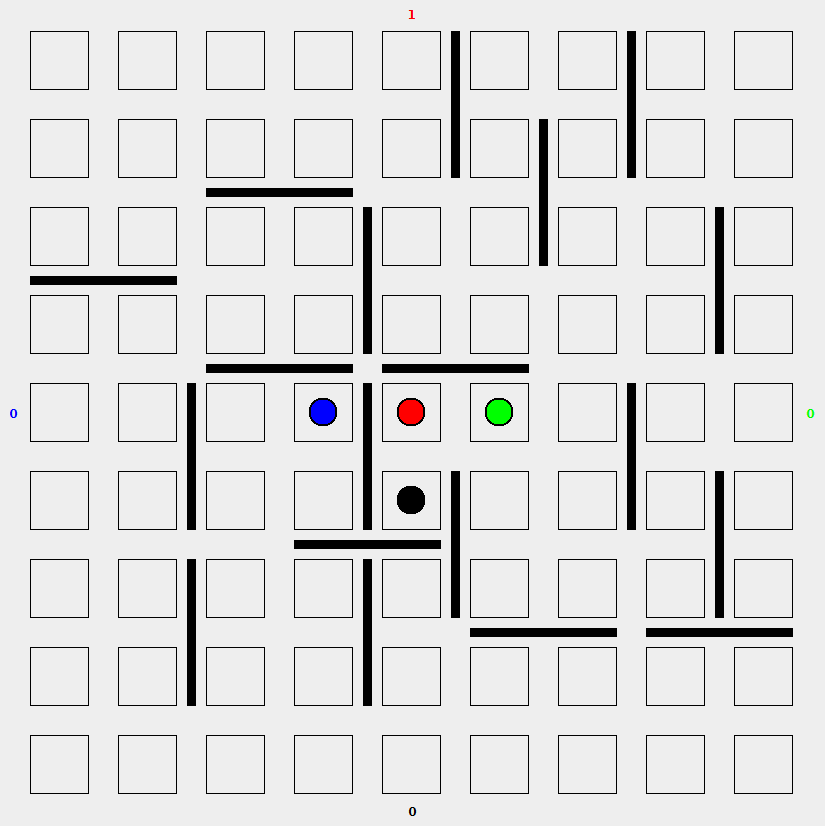
\includegraphics[width=80mm]{no-move.png}
\end{rysunek}

\subsection{Rozwiązanie problemu}

Zasady nie przewidują sytuacji, w której nie ma legalnych ruchów i żaden gracz nie zwyciężył.
Możliwe wyjścia z tej sytuacji to

\begin{enumerate}
\item \label{loose-turn} odebranie ruchu zablokowanemu graczowi
\item \label{loose-game} uznanie braku możliwych ruchów za porażkę
\item \label{prevent} zakazanie ruchu, który doprowadza do takiej sytuacji
\item \label{solve} dozwolonie dodatkowych ruchów
\end {enumerate}

Jedynym dostępnym kryterium przy dokonaniu wyboru jest tutaj subiektywna jakość rozgrywki, która powinna jak najlepiej przypominać oryginalną grę.
Rozwiązania \ref{loose-turn} i \ref{loose-game} naszym zdaniem nadto zmieniają zasady.
Pierwsze stwarza możliwość celowego blokowania gracza, aby układać ogrodzenia nie odczuwając kosztu związanego z nieporuszeniem pionka.
Drugie jest jeszcze większą ingerencją w dostępne strategie, ponieważ uznając więcej stanów za końcowe pozwala porzucić oryginalny cel rozgrywki, tzn. dotarcie na drugą stronę planszy.
Wadą wariantu numer \ref{prevent} jest mała przejrzystość.
Jeżeli jeden gracz wykona ruch pozostawiący następnemu tylko jeden możliwy ruch, który w efekcie odbierze trzeciemu wszystkie możliwości, ruch pierwszego gracza powinien być zakazany.
Jest to jednak trudne do spotrzeżenia i gracz pierwszy może nie rozumieć, dlaczego nie może wykonać takiego ruchu.

Wybraliśmy więc rozwiązanie \ref{solve}, poszerzając definicję przeskoczenia pionka przeciwnika.
Zgodnie z nową definicją gracz może przeskoczyć sąsiadujący (i nieodgrodzony) pionek przeciwnika stawiając swój  na dowolnym polu, na który mógłby postawić go przeciwnik, gdyby właśnie wykonywał ruch.
We wcześniej przedstawionym przykładzie, ruch wykonuje gracz czarny.
Gdyby ruch wykonywał gracz czerwony, mógłby przeskoczyć pionek gracza zielonego.
A zatem gracz czerwony również może to zrobić, co daje mu dwa możliwe ruchy do wyboru.

Ponieważ pierwotne zasady gry zapewniają, że każdy gracz ma dostępną przynamniej jedną drogę do celu, nowa definicja przeskoczenia pionka gwarantuje, że zawsze można wykonać ruch pionkiem.

\section{Interfejs bota}

Przed rozwijaniem algorytmów botów należy określić sposób w jaki będzie on udzielał odpowiedzi i ograniczenia, jakie zostaną narzucone.
Musimy tu przede wszystkim wziąć pod uwagę jakość użytkowania aplikacji i ograniczenia urządzeń, na jakich ma być uruchamiana.

Najprostszym interfejsem bota byłaby pojedyncza procedura, której jedynym argumentem jest stan gry, a wynikiem jest jeden z dozwolonych ruchów.
Utrudnia ona jednak właściwe wykorzystanie czasu.
Nie ma on możliwości wyboru decyzji jako wydającej się najlepszą w danej chwili i dalszego szukania lepszej.
Jeżeli próbując wykorzystać cały dostępny czas przekroczy go, arbiter przerwie procedurę i nie obliczy ona żadnego wyniku.

Dlatego jako interfejs bota obraliśmy procedurę nie mającą wyniku, która będzie uruchamiana przez aplikację w osobnym procesie na wyznaczony czas, a następnie przerywana.
Podczas działania będzie mogła modyfikować swoją decyzję o wybranym ruchu, będącą obiektem współdzielonym z procesem arbitra aplikacji.

Dla zapewnienia płynności rozgrywki, limit czasu ustalamy na 2 sekundy.
Oczywiście mógłby być konfigurowany przez użytkownika, ale wyszczególnienie pożądanej wartości pomoże w porównywaniu botów i wskazaniu algorytmu, który najlepiej sprawdza się w określonych warunkach.

Ustaliliśmy też przybliżone maksymalne zużycie pamięci na 500 MB, co ma znaczenie zwłaszcza dla algorytmów wykorzystujące tablicę transpozycji, która tym lepiej się sprawdza, im jest większa.
Jednak nasza aplikacja ma działać na współczesnym komputerze osobistym (który ma dziś zwykle 4 GB pamięci), a nie brać udział w potyczkach botów na superkomputerach.

\chapter{Rozwijanie botów}

\section{Minimax i Max\textsuperscript{n}}

Pierwszy zaimplementowany bot był oparty o Minimax i Max\textsuperscript{n} (w wersji dla czterech graczy).
Choć same algorytmy nie stwarzały problemów podczas implementacji, były pretekstem do opracowania procedury iteracyjnego pogłębiania i funkcji oceniającej, które miały być ponownie przydatne podczas pracy nad kolejnymi botami.

\subsection{Iteracyjne pogłębianie}

Zastosowanie techniki iteracyjnego pogłębiania miało na celu jak najlepsze wykorzstanie danego botowi czasu i zaprojektowanego dla niego interfejsu.
Oryginalny Minimax rozpatruje drzewo gry do ustalonej głębokości; przyjęcie zbyt małej wartości mogłoby oznaczać niższej jakości wynik obliczony w krótkim czasie, a zbyt wysokiej - przekroczenie limitu czasowego i brak jakiegokolwiek wyniku.
Iteracyjne pogłębianie polega na wielokrotnym wykonywaniu algorytmu, za każdym razem dla głębokości większej o 1 (co oznacza wykładniczy wzrost liczby rozpatrywanych stanów gry).

W procedurze iteracyjnego pogłębiania wprowadziliśmy dodatkowe usprawnienia, które miały poprawić jakość rozgrywki.
Chcieliśmy ograniczyć sytuacje, kiedy gracz komputerowy przekonany, że wygra (maksymalna wartość \(minimax\) korzenia) niespiesznie dąży do celu albo odwrotnie, gracz przekonany o porażce (minimalna wartość korzenia) poddaje się i nie zmierza nawet do celu licząc na błąd przeciwnika.
Oryginalny algorytm na równi traktuje ruchy prowadzące do pewnego zwycięstwa (analogicznie klęski), więc bot może przez wiele tur przesuwać pionek w tę i z powrotem, dopóki przeciwnik nie zbliży się odpowiednio do celu.
Przeciwnik z kolei może wcale nie zbliżać się do celu, również kręcąc się w kółko wobec wyboru między porażką w takiej czy innej liczbie ruchów.
Żeby ograniczyć takie sytuacje, spośród ruchów najlepszych z punktu widzenia wartości \(minimax\) wybieramy ten, który najbardziej zbliża do celu.
Ponad to, jeżeli wartość minimaks oznacza pewne zwycięstwo lub nieuchronną przegraną, pogłębianie jest przerywane, dzięki czemu bot szybciej wykonuje ruchy, zwłaszcza pod koniec rozgrywki.

\subsection{Funkcja oceniająca}

Do obliczania wartości funkcji oceniającej używamy pomocniczych wartości: odległości danego gracza do celu \(distance\), minimalnej odległości do celu przeciwników \(minOtherPlayerDistance\), ilości ścianek, jakie pozostały wybranemu graczowi \(wallsLeft\) oraz dwóch stałych: ilości ścianek w grze \(WALL\_COUNT\) (20) i górnego ograniczenia na długość najkrótszej ścieżki do celu \(DISTANCE\_UPPER\_BOUND\), za które przyjęliśmy liczbę pól planszy (81).
W przypadku stanów końcowy, funkcja przyjmuje skrajne wartości: \[-DISTANCE\_UPPER\_BOUND * WALL\_COUNT \text{,}\] \[(DISTANCE\_UPPER\_BOUND + 1) * WALL\_COUNT\] odpowiednio w przypadku porażki i zwycięstwa zadanego gracza.
W pozostałych przypadkach wynikiem jest \[(minOtherPlayerDistance - distance) * WALL\_COUNT + wallsfLeft \text{.}\]

Intuicyjnie, zgodnie z tą funkcją bot stara się mieć jak największą przewagę (lub najmniejszą stratę) w odglełości do celu względem najlepszego z przeciwników, a jeżeli jest to możliwe na wiele sposobów - zachowując jak najwięcej ścianek.
Łatwo zauważyć, że ma ona pożądane właściwości: skrajne wartości przyjmuje wtedy i tylko wtedy, gdy rozpatruje końcowy stan gry.
Co więcej, nadaje się też do ulepszania algorytmu Max\textsuperscript{n} analogicznie do Alfy-Bety, tzn. ma ograniczenie na sumę wartości dla wszystkich graczy, lepsze niż ograniczenie na wartość dla jednego gracza pomnożone przez ich liczbę.
Ograniczeniem tym jest \(WALL\_COUNT\).
W istocie, dla każdego stanu gracze wnoszą do sumy dwie składowe - przewagę nad najlepszym z przeciwników w odległości do celu i liczbę ścianek.
Suma drugich składników jest ograniczona właśnie przez \(WALL\_COUNT\), a suma pierwszch przez \(0\) - dla dwóch graczy najbliższych celowi są to liczby przeciwne, a dla pozostałych niedodatnie.

\section {Alfa-Beta}

Drugim zaimplementowanym algorytmem był Alfa-Beta.
Wersja właściwa, dla dwóch graczy, nie stworzyła problemów implementacyjnych.
Natomiast samo wprowadzenie odcięć (porzucanie niektórych poddrzew), nakłoniło nas do ulepszenia implementacji zasad gry w celu przyspieszenia tego bota i wykonania przez niego większej liczby iteracji.
Chodziło o stopniowe obliczanie możliwych ruchów, w miejsce wyznaczania ich wszystkich od razu.
W wielu grach mogłoby to nie mieć znaczenia, jednak w Quoridor sprawdzenie legalności postawienia ściany wymaga upewnienia się, że każdy przeciwnik wciąż ma drogę do celu.
Do tego potencjalnie możliwych ruchów tego rodzaju na począku gry jest ponad sto, a rozpatrywanie legalnych ruchów jest częstą operacją dla każdego z botów.
Dlatego postanowiliśmy wyznaczać legalne ruchy po jednym, licząc na to, że po odcięciu poddrzewa sprawdzanie ruchów ścianką nie będzie potrzebne, a przynajmniej będzie ograniczone.
Co więcej, ruchy, których legalność łatwiej zweryfikować, zaczęliśmy rozpatrywać jako pierwsze.
Dodaliśmy też specjalną obsługę kilku przypadków, w których można szybciej stwierdzić, że każdy ma drogę do celu (np. wszystkie ściany na planszy są ustawione w tym samym kierunku).

Wersję dla czterech graczy udoskonaliliśmy.
Opisany wcześniej algorytm obliczał \(bound\) na podstawie dwóch dodatkowych, danych wraz z funkcją oceniającą wartości: dolnego ograniczenia na każdy element wektora wartości (autorzy przyjęli 0, ponieważ można przesunąć wartości) i górnego na sumę liczb w wektorze \(sum\).
Jeżeli osiągalnej dla jednego gracza \(value\) odpowiadało \(bound\) (równe \(sum - value\)), to osiągnięcie przez kolejnego gracza w następnym ruchu \(bound\) lub więcej oznaczało, że pierwszemu graczowi pozostawia to wynik najwyżej \(value\), a więc całe poddrzewo wynikające z takiego ruchu można porzucić.

Przyjęta przez nas funkcja oceniająca ma dodatkową właściwość: suma każdych dwóch liczb w wektorze wartości jest ograniczona z góry (przez \(WALL\_COUNT\)).
Dla stanów końcowych jest to oczywiste.
W pozostałych stanach dwaj gracze najbliżsi celu są dla siebie nawzajem przeciwnikami o minimalnej odległości do celu, więc suma wartości funkcji oceniającej dla każdego z nich to łączna liczba płytek stanowiąca ich zasoby.
Każda inna para graczy daje sumę jeszcze mniejszą.

A zatem za \(bound\) możemy przyjąć \(WALL\_COUNT - value\), a nie jedynie \[WALL\_COUNT + 2 * DISTANCE\_UPPER\_BOUND * WALL\_COUNT - value\text{,}\] co daje oryginalne podejście w wersji dla czterech graczy.

\section{Tablica transpozycji}

Spośród możliwych ulepszeń algorytmów Minimax Alfa-Beta wybraliśmy do zaimplementowania tablicę transpozycji jako to, które nadaje się do zastosowania wobec wersji dla wielu graczy opartej o Max\textsuperscript{n}.
Użycie tej techniki wymagało po pierwsze zaprojektowania funkcji haszującej, do czego użyliśmy metody znanej jako haszowanie Zobrista, po drugie metody użycia wobec Alfy-Bety dla wielu graczy.
O ile przykłady użycia tablicy transpozycji zarówno dla algorytmu Minimax i Alfa-Beta w standardowej, dwuosobowej wersji są łatwo dostępne, a przypadek Max\textsuperscript{n} jest w zasadzie identyczny co Minimax, o tyle Alfa-Beta dla wielu graczy w oparciu o Max\textsuperscript{n} została opracowana przez nas samodzielnie (co oczywiście nie oznacza, że pioniersko).

\subsection{Haszowanie Zobrista}

Projektując funkcję haszującą techniką Zobrista, najpierw należy rozkłożyć stan gry na składowe.
W naszym przypadku były to (załóżmy przypadek czteroosobowy):

\begin{itemize}
\item indeks gracza, który właśnie wykonuje ruch (\(p \in \{0, 1, 2, 3\}\))
\item stan każdego z \(8 \times 8\) skrzyżowań szczelin na planszy: 1 dla środka ogrodzenia poziomego, 2 dla pionowego, 0 w przeciwnym wypadku (\( b_{0, 0}, b_{0, 1}, .., b_{0, 7}, b_{1, 0}, .., b_{7, 7} \in \{0, 1, 2\}\))
\item pozycja pionka każdego gracza (\(x_0, y_0, x_1, y_1, x_2, y_2, x_3, y_3 \in \{0, 1, .., 8\}\))
\item liczba ogrodzeń stanowiących zasoby graczy (\(w_0, w_1, w_2, w_3 \in \{0, 1, 2, 3, 4, 5\}\))
\end {itemize}

Otrzymaliśmy więc 150 zmiennych, których wartości wzajemnie jednoznacznie wyznaczały stany gry.
Dalej, dla tych zmiennych \(v_0, v_1, .., v_{149}\) utworzyliśmy tablice \(V_0, V_1, .., V_{149}\) tak, żeby długość \(V_i.length\) każdej tablicy była równa liczbie wartości przyjmowanych przez odpowiadającą zmienną \(v_i\).
Dalej, losowo wypełniliśmy te tablice liczbami z przedziału właściwego dla typu ich elementów (wybraliśmy \emph{long} z języka Java).

Wtedy już mogliśmy zdefiniować wartość funkcji haszującej \(h(s)\) dla stanu \(s\) opisanego wartościami zmiennych \(v_0, v_1, .., v_{149}\) jako \[\oplus_{i = 0}^{149} V_i[v_i]\text{,}\] gdzie znak \(\oplus\) oznacza binarną operację XOR (alternatywę rozłączną).

Funkcja haszująca zaprojektowana techniką Zobrista daje się ponadto obliczać inkrementalnie, to znaczy znając jej wartość dla danego stanu i wykonany po nim ruch można wydajniej obliczyć wartość dla stanu wynikowego.
Wykorzystuje się tu fakt, że operacja XOR jest łączna, przemienna i każdy element jest sam wobec siebie odwrotny.
W przypadku Quoridor, wykonanie ruchu zmienia wartość najwyżej trzech zmiennych wykorzystanywanych do opisu stanu.
Jedną z nich jest zawsze indeks gracza wykonującego ruch.
Dla ruchu pionkiem, pozostałe to pozycja pionka gracza wykonującego ruch.
W przypadku postawienia ogrodzenia, są to liczba pozostałych graczowi ogrodzeń i stan tego ze skrzyżowań szczelin planszy, na którym znalazł się środek ogrodzenia.
Jeżeli dla każdej zmiennej \(v_i\), która w wyniku ruchu zmieniła wartość z \(x_i\) na \(y_i\) zastosujemy wobec wartość funkcji haszującej dla wyjściowego stanu operację XOR z \(V_i[x_i] \oplus V_i[y_i]\), otrzymamy wartość funkcji haszującej dla stanu wynikowego.
A więc rozpatrzymy jedynie 3 zmienne zamiast 150.

Przypadek dla dwóch graczy wymaga niewielkich zmian: znikają zmienne \(x_2\), \(x_3\), \(y_2\), \(y_3\), \(w_2\), \(w_3\), ponadto \(p \in \{0, 1\}\) i \(w_0, w_1 \in \{0, 1, .., 10\}\).

\subsection{Zastosowanie wobec Alfy-Bety dla wielu graczy}

Przypomnijmy, że Max\textsuperscript{n} przypisuje stanom gry wektor, którego składowe to wartości funkcji oceniających dla każdego z graczy.
Ulepszenia analogiczne do Alfy-Bety wprowadza do rozpatrywania wierzchołka dodatkowy parametr \(bound\), który ogranicza z góry wartości odpowiadające graczowi wykonującemu ruch tak samo, jak \(beta\) dla gracza \(max\) w wersji dwuosobowej.

Ponieważ \(bound\) odwołuje się do aktualnego gracza, nasze użycie tablicy transpozycji dla tego algorytmu opiera się na założeniu, że wartość funkcji haszującej zależy od gracza wykonującego ruch, co być może nie jest konieczne w innych przypadkach.
Opisana wcześniej funkcja haszująca spełnia ten warunek.

Wpis w tablicy transpozycji wyposażyliśmy w następujące pola:

\begin{itemize}
\item{\(hash\): wartość funkcji haszującej, jest wykorzystywana do weryfikacji adekwatności wpisu. Można go użyć tylko, jeżeli \(hash\) jest równe wartości funkcji haszującej rozpatrywanego stanu gry.}
\item{\(depth\): odległość od liści w drzewie przeszukiwania z momentu tworzenia wpisu, używana jako wskaźnik jakości. Wpisu można użyć tylko, jeżeli \(depth\) jest większe lub równe aktualnej odległości od liści.}
\item{\(exact\): wartość logiczna, która określa czy pole \(value\) to dokładny wektor wartości, czy tylko osiągalny z punktu widzenia gracza wykonującego ruchu.}
\item{\(value\): wektor wartości funkcji oceniającej dla graczy.}
\end{itemize}

Rozpatrując wierzchołek, nasz algorytm najpierw odnajduje właściwy mu wpis w tablicy transpozycji i jeśli go znajdzie, sprawdza czy wartości \(hash\) i \(depth\) pozwalają go użyć.
Jeżeli tak, oraz jest to wpis dokłady (\(exact\) jest prawdą) albo wartość w wektorze odpowiadająca aktualnemu graczowi przekracza \(bound\), odnaleziona \(value\) jest używana jako wynik bez dalszych obliczeń.

Kiedy wpis nie zostanie odnaleziony albo nie okaże się przydatny, algorytm oblicza wynik tak samo, jak bez użycia tablicy transpozycji.

Na końcu procedury, jeżeli wpis nie został wcześniej odnaleziony albo został odrzucony z powodu niewłaściwych wartośc \(hash\) czy \(depth\), do tablicy zapisywany jest nowy wpis.
Obliczony wynik trafia do \(value\), a wartość \(exact\) ustala się jako prawdę wtedy i tylko wtedy, gdy wartość w wektorze wynikowym odpowiadającemu graczowi jest mniejsza niż \(bound\).

Postępowanie z \(hash\) i \(depth\) niczym nie różni się tutaj od standardowej, dwuosobowej wersji algorytmu Minimax z tablicą transpozycji.
Więcej uwagi wymagają specyficznie używane \(exact\) i \(value\).

Jeżeli \(exact\) jest prawdą, wpis należy odczytywać następująco: ,,wektor wartości dla odpowiadającego stanu został dokładnie obliczony, znajduje się w \(value\)'', więc \(value\) natychmiast przyjmujemy ją za wynik, tak jakbyśmy wykonywali Max\textsuperscript{n} z użyciem tablicy transpozycji.

Dopiero kiedy \(exact\) jest fałszem, widoczne jest działanie \(bound\) - wpis oznacza, że ,,jeden z synów ma wartość \(value\), a więc ten stan jest co najmniej równie dobry z punktu widzenia gracza wykonującego ruch''. Dokładna wartość nie została obliczona, ponieważ już \(value\) przekroczyło \(bound\) używane w trakcie tworzenia wpisu.
Co więcej, takie znaczenie wpisu może być użyteczne tylko jeżeli jest jasne o którego gracza chodzi, stąd dodatkowe wymaganie dla funkcji haszującej.
Takiego wpisu możemy użyć tylko jeżeli wynik nie musi być dokładny, a więc gdy \(value\) przekracza aktualne \(bound\).

\section{Monte Carlo Tree Search}

Zgodnie z wcześniejszym opisem algorytmu Monte Carlo Tree Search (dales ,,MCTS''), zaimplementowany przez nas MCTSBot był parametryzowany sposobem obliczania współczynnika ufności \(hopeFactor\), \(\sqrt{\frac{\sqrt{n_p}}{n_s}}\) lub \(\sqrt{\frac{\log{n_p}}{n_s}}\), które będziemy nazywać odpowiednio \(SQRT\) i \(LOG\), oraz liczbą symulacji po której rozwijany jest liść \(expansionThreshold\), która zwykle jest zbliżona do liczby możliwych ruchów (dla Quoridor jest to maksymalnie 138, minimalnie 1).
Podczas pierwszych obserwacji tego bota zauważyliśmy, że bez względu na dobór parametrów wydaje się wybierać losowe ruchy.
W przyjętym przez nas limicie czasowym na ruch wykonywał zbyt mało symulacji, często nie rozwijając żadnego liścia.
Żeby temu zabopiec, postanowiliśmy skrócić symulacje, wprowadzając kolejny parametr: limit długości symulacji \(maxMoves\).
Po osiągnięciu tej wartości zwyciężcę symulacji algorytm miał wyłaniać na podstawie odległości do celu.
Udało się nam zaobserwować poprawę i wytypować kandydatów na wartości dla wszystkich parametrów.

\subsection{Metoda optymalizacji parametrów}

Do pierwszej serii eksperymentów mających na celu wyznaczenie optymalnych wartości parametrów wybraliśmy 2 wartości dla \(hopeFactor\) (\(LOG\) i \(SQRT\)), 4 dla \(expansionThreshold\) (40, 80, 120 i 160) i 4 dla \(maxMoves\) (3, 5, 7, 9), czyli 32 kombinacje.

Przy przeprowadzaniu automatycznych turniejów należało zadbać o to, żeby zachować symetrię i nie dać żadnemu botowi przewagi umieszczając go częściej na którejś pozycji, np. jako rozpoczynającego.
Prostym sposobem na spełnienie tego warunku jest rozpatrzenie wszystkich możliwych konfiguracji, ale przy 32 algorytmach i 4 graczach przekracza to nasze możliwości obliczeniowe.
Dlatego zdecydowaliśmy się nie porównywać różnych wariantów MCTS do siebie bezpośrednio, ale każdego z osobna do bota Minimax (który, przypomnijmy, wykonuje Max\textsuperscript{n} w wersji dla czterech graczy).
Wszystkich możliwych sposobów przypisania jednego dwóch algorytmów do \(k\) kolejnych graczy tak, by jeden nie sterował wszystkimi, jest \(2^k - 2\).
Tak więc każdy MCTSBot miał rozegrać przeciw Minimaksowi jednakową liczbę meczy dwuosobowych w każdej z \(2^2 -2 = 2\) kombinacji, oraz jednakową liczbę meczy czteroosobowych w każdej z \(2^4 - 2 = 14\) kombinacji.
Miarą skuteczności parametrów miała być liczba zwycięstw, rozpatrywana osobno dla obu wariantów gry.
W związku z rozdzieleniem eksperymentów względem liczby graczy, spodziewaliśmy się otrzymać różne zestawy parametrów, które potem miały zostać wykorzystane w jednym bocie, przyjmującym jedne lub drugie parametry w zależności od wariantu gry.

\subsection{Optymalizacja parametrów dla wersji dwuosobowej}

W przypadku wersji dwuosobowej, dla każdej kombinacji parametrów pierwszego zestawu przeprowadziliśmy 25-krotnie mecze z Minimaksem we obu możliwych ustawieniach, a więc każdy wariant MCTS rozegrał 50 pojedynków.
Rysunek \ref{experiment1-2p}. podsumowuje uzyskane wyniki, w pełni przedstawione w dodatku \ref{results-1-2p}.

\begin{rysunek}
\caption{Wyniki eksperymentów z parametrami MCTS (2 graczy, zestaw 1) \label{experiment1-2p}}
\centering
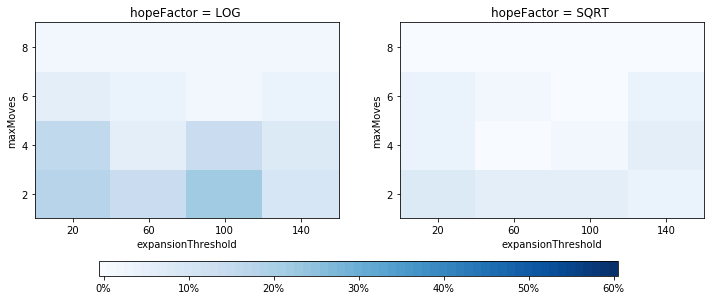
\includegraphics[width=160mm]{experiment1-2p.png}
\end{rysunek}

W drugiej serii eksperymentów postanowiliśmy rozpatrzeć wyłącznie \(hopeFactor = LOG\), 5 wartości \(expansionThreshold\) (20, 40, 60, 80, 100) i 3 wartości maxMoves (1, 2, 3).
Rysunek \ref{experiment2-2p}. podsumowuje uzyskane wyniki, w pełni przedstawione w dodatku \ref{results-2-2p}.

\begin{rysunek}
\caption{Wyniki eksperymentów z parametrami MCTS (2 graczy, zestaw 2) \label{experiment2-2p}}
\centering
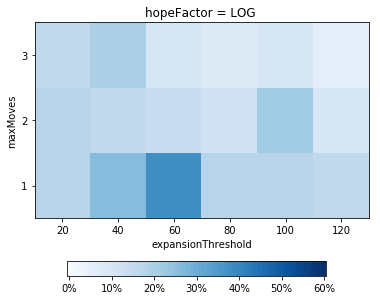
\includegraphics[width=80mm]{experiment2-2p.png}
\end{rysunek}

Ostatecznie, dla wersji dwuosobowej ustaliliśmy parametry \[hopeFactor = LOG, expansionThreshold = 60, maxMoves=1,\] które dały zwycięstwo nad Minimaksem w 19 rozgrywkach na 50.

\subsection{Optymalizacja parametrów dla wersji czteroosobowej}

W przypadku wersji czteroosobowej, dla każdej kombinacji parametrów pierwszego zestawu przeprowadziliśmy 5-krotnie mecze z Minimaksem we wszystkich czternastu możliwych ustawieniach, a więc każdy wariant MCTS rozegrał 70 pojedynków.
Rysunek \ref{experiment1-4p}. podsumowuje uzyskane wyniki, w pełni przedstawione w dodatku \ref{results-1-4p}.

\begin{rysunek}
\caption{Wyniki eksperymentów z parametrami MCTS (4 graczy, zestaw 1) \label{experiment1-4p}}
\centering
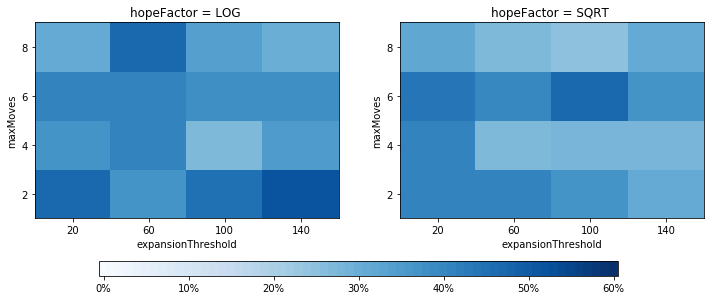
\includegraphics[width=160mm]{experiment1-4p.png}
\end{rysunek}

W drugiej serii eksperymentów postanowiliśmy rozpatrzeć wyłącznie \(hopeFactor = LOG\), 10 wartości \(expansionThreshold\) (20, 40, 60, 80, 100, 120, 140, 160, 180, 200) i 3 wartości maxMoves (1, 2, 3).
Rysunek \ref{experiment3-4p}. podsumowuje uzyskane wyniki, w pełni przedstawione w dodatku \ref{results-3-4p}.

\begin{rysunek}
\caption{Wyniki eksperymentów z parametrami MCTS (4 graczy, zestaw 3) \label{experiment3-4p}}
\centering
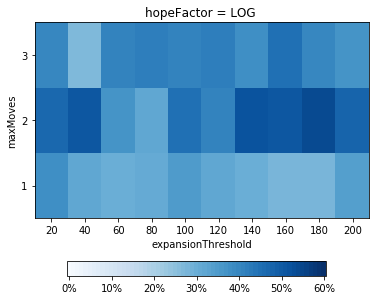
\includegraphics[width=80mm]{experiment3-4p.png}
\end{rysunek}

Ostatecznie, dla wersji czteroosobowej ustaliliśmy parametry \[hopeFactor = LOG, expansionThreshold = 180, maxMoves=2,\] które dały zwycięstwo nad Minimaksem w 38 rozgrywkach na 70.

\chapter{Podsumowanie}

\section{Porównanie zaimplementowanych algorytmów}

Po zaimplementowaniu botów, przeprowadziliśmy automatyczny turniej w celu porównania ich i sprawdzenia, czy ulepszenia rzeczywiście okazały się skuteczne.
Wzięły w nim udział boty

\begin{itemize}
    \item \(AlphaBetaTT\) - Alfa-Beta z tablicą transpozycji (dla wersji czteroosobowej odpowiednik oparty na Max\textsuperscript{n})
    \item \(Minimax\) - Minimax (w wersji czteroosobowej Max\textsuperscript{n})
    \item \(MCTS\) - Monte Carlo Tree Search, z parametrami ustalonymi wcześniej ekserymentalnie, osobno dla obu wersji gry
\end{itemize}

Ze względu na małą liczbę uczestników, możliwe było wieloktrotne przeprowadzenie meczy we wszystkich możliwych ustawieniach, w których graczami sterują co najmniej dwa różne algorytmy.
W przypadku rozgrywki dwuosobowej jest to \(3^2 - 3 = 6\) kombinacji, dla czteroosobowej \(3^4 - 3 = 78\).
Te pierwsze powtarzaliśmy 65 razy, a drugie 5, a więc dla obu wersji przeprowadziliśmy 390 meczy.

Oba warianty gry dały ten porządek uczestników turnieju według skuteczności (por. z tabelą \ref{turniej}).
\(AlphaBetaTT\), zgodnie z oczekiwaniami, okazał się lepszy od bota \(Minimax\), którego jest ulepszeniem.
\(MCTS\) dwukrotnie zajął ostatnie miejsce, wyraźnie mniej skuteczny w rozgrywce dwuosobowej i bliższy pozostałym w czteroosobowej.

\begin{tabela}
    \caption{Wyniki turnieju podsumowującego \label{turniej}}
    \begin{tabular}{| c | c | c | c |}
	\hline
        bot & liczba zwycięstw w grze dwuosobowej & liczba zwycięstw w grze czteroosobowej \\ \hline
	\hline
        AlphaBetaTT & 176 & 141 \\ \hline
        Minimax & 167 & 132 \\ \hline
        MCTS & 47 & 117 \\ \hline
    \end{tabular}
\end{tabela}

\section{Efekty ogólne}

Spośród metod opracowanych przez nas samodzielnie, dwie są dość ogólne, by użyć ich wobec innych gier.
Obiema zajmowaliśmy się na potrzeby czteroosobowego wariantu Quoridor, ale mogą być przydatne przy każdej liczbie graczy większej niż dwa - dla gier dwuosobowych pozostają poprawne, jednak mniej efektywne od swoich powszechnie stosowanych odpowiedników specyficznych dla klasycznego pojedynku.

Pierwszą z nich jest inne, umożliwiające większą ilość odcięć, obliczanie \(bound\) przy implementacji analogicznego do Alfy-Bety ulepszenia dla Max\textsuperscript{n}, możliwe dzięki wzmocnieniu założenia na temat funkcji oceniającej.
Przypomnijmy, że wymaga to istnienia górnego ograniczenia na sumę każdych dwóch liczb w wektorze wartości, silniejszego niż to, które wynika z ograniczenia górnego na sumę wszystkich liczb w tym wektorze, wymaganego w oryginalnej wersji.
Takiego ograniczenia możemy się spodziewać, jeżeli funkcja oceniająca dba tylko o sytuację gracza względem najlepiej usytuowanego przeciwnika.
Jest to naturalne w przypadku gier wyłaniających i nagradzających wyłącznie jednego zwyciężcę.

Drugim takim efektem naszej pracy jest sposób zastosowania tablicy transpozycji wobec wieloosobowej Alfy-Bety.
Ponieważ wartość \(bound\), będąca elementem wpisu tablicy, sama w sobie nie informuje którego gracza dotyczy, podkreśliliśmy wymóg, by funkcja haszująca brała pod uwagą gracza wykonującego ruch.
Warunek ten jest bardzo naturalny i trudno nam odnaleźć grę, w którym nie był konieczny z innych powodów.

\section{Wypełnienie założeń}

Dzięki zaimplementowanym botom, wytworzony przez nas prototyp aplikacji, zgodnie z założeniami, pozwala obserwować i mierzyć się z różnymi algorytmami.
Zgodnie z planem kod źródłowy jest dostępny publicznie, z wyodrębionymi częściami odpowiedzialnymi za zasady gry, sztuczną inteligencję, aplikację i narzędzia do przeprowadzania eksperymentów (por. dodatek \ref{code}), co umożliwia zrozumienie i ulepszanie działania botów.

Wybranie języka Java do implementacji zapewniło łatwość dystrybucji.
Projekt pozwala jednym poleceniem zbudować plik JAR, niezależny od architektury i wykonywalny na popularnych systemach operacyjnych, które standardowo wspierają środowisko uruchomieniowe Javy.
Modularna budowa i dobór technologii umożliwia też przyszłe wytworzenie aplikacji na urządzenia mobilne z systemem Android, z wykorzystaniem tego samego kodu odpowiedzialnego za zasady gry i sztuczną inteligencję.

Poziom samych botów, odczuwany subiektywnie podczas rozgrywki, możemy określić jako zadowalający, jednak nie dość wysoki, by użyć któregoś jako poziom ,,bardzo trudny'' w aplikacji dla użytkownika niezainteresowanego algorytmami.
Może być to konsekwencja rygorystycznego limitu na czas jak na grę z dużą liczbą możliwych ruchów i wyboru technologii.
Chcielibyśmy jednak wskazać kierunki poszukiwań dla poprawy, inne niż zwiększanie limitu czasowego.

\section{Kierunki dalszego rozwoju sztucznej inteligencji}

Bez względu na algorytm sterujacy botem, kilka pierwszych ruchów można potraktować specjalnie, implementując kilka otwarć uznanych za dobre.
Losowanie jednego z nich przez rozpoczynającego grę może też urozmaicić rozgrywkę, zwłaszcza w przypadku metod deterministycznych, dla których jedynym źródłem losowości jest moment przerwania obliczeń z powodu przekroczenia limitu czasowego.

Dalsze ulepszanie \(AlphaBetaTT\) mogłoby polegać na manipulowaniu oknem przeszukiwań / \(bound\).
O ile w przypadku gry dwuosobowej jest to dobrze opracowana i skuteczna metoda, o tyle wersja czteroosobowa jest nie tylko nieopisana, ale i nie jest jasne, czy byłaby skuteczna.
Pamiętajmy, że samo \(bound\) pozwala na mniej odcięć niż okno przeszukiwań, a nieudana próba skrócenia obliczeń oznacza zmarnowanie czasu.

Poprawianie Monte Carlo Tree Search może polegać na manipulowaniu parametrami w trakcie gry (ilość możliwych ruchów drastycznie spada, a jest to punkt wyjścia do poszukiwania \(expensionThreshold\)).
Innym kierunkiem byłaby zmiana rozkładu prawdopodobieństwa wyboru ruchu podczas losowania, który bez zastosowania wiedzy eksperckiej jest jednostajny.

\begin{thebibliography}{98}
\addcontentsline{toc}{chapter}{Bibliografia}

\bibitem[1]{anderson} Eike Anderson, \textit{Playing smart - artificial intelligence in computer games}, materiał na konferencję zfxCON03, 2003
\bibitem[2]{mertens} P.J.C Mertens, \textit{A Quoridor-playing Agent},\\https://project.dke.maastrichtuniversity.nl/games/files/bsc/Mertens\_BSc-paper.pdf, 2006
\bibitem[3]{pawlewicz} Jakub Pawlewicz, \textit{Techniki sztucznej inteligencji
    w programach grających}, https://www.mimuw.edu.pl/\textasciitilde{}pan/gry.pdf, 2010
\bibitem[4]{sturtevant} Nathan Reed Sturtevant, \textit{Multi-Player Games: Algorithms and Approaches}, University of California Los Angeles, 2003
\bibitem[5]{korf} Richard Korf, \textit{Multi-player alpha-beta pruning}, Artificial Intelligence, vol. 48 no. 1, 1991

\end{thebibliography}

\begin{appendices}

    \chapter{Kod źródłowy aplikacji \label{code}}

    Na dołączonej płycie znajduje się wykonywalny plik \textit{quoridor-gui.jar} uruchamiający wytworzoną aplikację oraz katalog \textit{src} z kodem źródłowym, podzielonym jest na:

\begin{itemize}
    \item \textit{quoridor-core} - zasady gry, z kluczową klasą \textit{GameRules} w pliku \\ \textit{quoridor-core/src/main/java/quoridor/core/GameRules.java}
    \item \textit{quoridor-ai} - sztuczną inteligencję, z implementacją botów w katalogu \\ \textit{quoridor-ai/src/main/java/quoridor/ai/bot}
    \item \textit{quoridor-analysis} - narzędzia do przeprowadzania automatycznych rozgrywek między botami
    \item \textit{quoridor-gui} - aplikację z interfejsem graficznym
\end{itemize}

    Bezpośrednio w katalogu \textit{src} znajduje się plik \textit{README.md} z któtkim opisem projektu i wskazówkami dotyczącymi rozwijania, w szczególności podaje sposób użycia znajdującego się obok skryptu \textit{gradlew} w celu zbudowania pliku wykonywalnego aplikacji.

\chapter{Pełne wyniki eksperymentów}

\section{Optymalizacja parametrów MCTS, 2 graczy, zestaw 1\label{results-1-2p}}

\begin{center}
    \begin{tabular}{| c | c | c | c |}
	\hline
    hopeFactor & expansionThreshold & maxMoves & liczba zwycięstw (na 50 meczy) \\ \hline
	\hline
        LOG & 100 & 2 & 11 \\ \hline
        LOG & 20 & 2 & 9 \\ \hline
        LOG & 20 & 4 & 8 \\ \hline
        LOG & 60 & 2 & 7 \\ \hline
        LOG & 100 & 4 & 7 \\ \hline
        LOG & 140 & 2 & 5 \\ \hline
        SQRT & 20 & 2 & 4 \\ \hline
        LOG & 140 & 4 & 4 \\ \hline
        LOG & 60 & 4 & 3 \\ \hline
        SQRT & 60 & 2 & 3 \\ \hline
        SQRT & 100 & 2 & 3 \\ \hline
        LOG & 20 & 6 & 3 \\ \hline
        SQRT & 140 & 4 & 3 \\ \hline
        SQRT & 140 & 2 & 2 \\ \hline
        SQRT & 20 & 4 & 2 \\ \hline
        LOG & 60 & 6 & 2 \\ \hline
        SQRT & 20 & 6 & 2 \\ \hline
        SQRT & 140 & 6 & 2 \\ \hline
        LOG & 140 & 6 & 2 \\ \hline
        SQRT & 60 & 6 & 1 \\ \hline
        LOG & 100 & 6 & 1 \\ \hline
        SQRT & 100 & 4 & 1 \\ \hline
        LOG & 100 & 8 & 1 \\ \hline
        LOG & 20 & 8 & 1 \\ \hline
        LOG & 60 & 8 & 1 \\ \hline
        LOG & 140 & 8 & 1 \\ \hline
    \end{tabular}
\end{center}

\vfill
\hspace{0pt}
\pagebreak

\section{Optymalizacja parametrów MCTS, 2 graczy, zestaw 2\label{results-2-2p}}

\begin{center}
    \begin{tabular}{| c | c | c | c |}
	\hline
    hopeFactor & expansionThreshold & maxMoves & liczba zwycięstw (na 50 meczy) \\ \hline
	\hline

        LOG & 60 & 1 & 19 \\ \hline
        LOG & 40 & 1 & 13 \\ \hline
        LOG & 100 & 2 & 11 \\ \hline
        LOG & 40 & 3 & 10 \\ \hline
        LOG & 20 & 1 & 9 \\ \hline
        LOG & 80 & 1 & 9 \\ \hline
        LOG & 20 & 2 & 9 \\ \hline
        LOG & 100 & 1 & 9 \\ \hline
        LOG & 20 & 3 & 8 \\ \hline
        LOG & 40 & 2 & 8 \\ \hline
        LOG & 120 & 1 & 8 \\ \hline
        LOG & 60 & 2 & 7 \\ \hline
        LOG & 80 & 2 & 6 \\ \hline
        LOG & 60 & 3 & 5 \\ \hline
        LOG & 120 & 2 & 5 \\ \hline
        LOG & 100 & 3 & 5 \\ \hline
        LOG & 80 & 3 & 4 \\ \hline
        LOG & 120 & 3 & 3 \\ \hline

    \end{tabular}
\end{center}

\vfill
\hspace{0pt}
\pagebreak

\section{Optymalizacja parametrów MCTS, 4 graczy, zestaw 1\label{results-1-4p}}

\begin{center}
    \begin{tabular}{| c | c | c | c |}
	\hline
    hopeFactor & expansionThreshold & maxMoves & liczba zwycięstw (na 70 meczy) \\ \hline
	\hline
        LOG & 140 & 2 & 37 \\ \hline
        LOG & 20 & 2 & 33 \\ \hline
        LOG & 60 & 8 & 33 \\ \hline
        SQRT & 100 & 6 & 33 \\ \hline
        LOG & 100 & 2 & 32 \\ \hline
        SQRT & 20 & 6 & 31 \\ \hline
        LOG & 20 & 6 & 29 \\ \hline
        SQRT & 20 & 2 & 29 \\ \hline
        SQRT & 20 & 4 & 29 \\ \hline
        LOG & 60 & 4 & 29 \\ \hline
        LOG & 60 & 6 & 29 \\ \hline
        SQRT & 60 & 2 & 29 \\ \hline
        SQRT & 60 & 6 & 28 \\ \hline
        LOG & 100 & 6 & 27 \\ \hline
        LOG & 140 & 6 & 27 \\ \hline
        LOG & 20 & 4 & 26 \\ \hline
        LOG & 60 & 2 & 26 \\ \hline
        SQRT & 100 & 2 & 26 \\ \hline
        SQRT & 140 & 6 & 26 \\ \hline
        LOG & 140 & 4 & 25 \\ \hline
        LOG & 100 & 8 & 24 \\ \hline
        SQRT & 20 & 8 & 23 \\ \hline
        LOG & 20 & 8 & 22 \\ \hline
        SQRT & 140 & 2 & 22 \\ \hline
        SQRT & 140 & 8 & 22 \\ \hline
        LOG & 140 & 8 & 21 \\ \hline
        SQRT & 100 & 4 & 20 \\ \hline
        SQRT & 140 & 4 & 20 \\ \hline
        SQRT & 60 & 4 & 19 \\ \hline
        SQRT & 60 & 8 & 19 \\ \hline
        LOG & 100 & 4 & 19 \\ \hline
        SQRT & 100 & 8 & 18 \\ \hline

    \end{tabular}
\end{center}

\vfill
\hspace{0pt}
\pagebreak

\section{Optymalizacja parametrów MCTS, 4 graczy, zestaw 3\label{results-3-4p}}

\begin{center}
    \vspace{0pt}
    \begin{tabular}{| c | c | c | c |}
	\hline
    hopeFactor & expansionThreshold & maxMoves & liczba zwycięstw (na 70 meczy) \\ \hline
        LOG & 180 & 2 & 38 \\ \hline
        LOG & 140 & 2 & 37 \\ \hline
        LOG & 40 & 2 & 36 \\ \hline
        LOG & 160 & 2 & 36 \\ \hline
        LOG & 200 & 2 & 34 \\ \hline
        LOG & 20 & 2 & 33 \\ \hline
        LOG & 100 & 2 & 32 \\ \hline
        LOG & 160 & 3 & 32 \\ \hline
        LOG & 80 & 3 & 30 \\ \hline
        LOG & 120 & 3 & 30 \\ \hline
        LOG & 60 & 3 & 29 \\ \hline
        LOG & 100 & 3 & 29 \\ \hline
        LOG & 120 & 2 & 29 \\ \hline
        LOG & 20 & 3 & 28 \\ \hline
        LOG & 180 & 3 & 28 \\ \hline
        LOG & 20 & 1 & 27 \\ \hline
        LOG & 140 & 3 & 27 \\ \hline
        LOG & 60 & 2 & 26 \\ \hline
        LOG & 200 & 3 & 26 \\ \hline
        LOG & 100 & 1 & 25 \\ \hline
        LOG & 200 & 1 & 24 \\ \hline
        LOG & 40 & 1 & 23 \\ \hline
        LOG & 80 & 2 & 23 \\ \hline
        LOG & 120 & 1 & 23 \\ \hline
        LOG & 80 & 1 & 22 \\ \hline
        LOG & 60 & 1 & 21 \\ \hline
        LOG & 140 & 1 & 21 \\ \hline
        LOG & 160 & 1 & 20 \\ \hline
        LOG & 180 & 1 & 20 \\ \hline
        LOG & 40 & 3 & 19 \\ \hline
    \end{tabular}
\end{center}

\end{appendices}

\end{document}


%%% Local Variables:
%%% mode: latex
%%% TeX-master: t
%%% coding: utf-8
%%% End:
